% 1. documento
\documentclass[12pt,a4paper]{article}

% 2. idioma y fuente
\usepackage[utf8]{inputenc}
\usepackage[T1]{fontenc}
\usepackage[spanish]{babel}

% 3. margenes
\usepackage[
    left=2.5cm,
    right=2.5cm,
    top=2cm,
    bottom=2cm
]{geometry}

% 4. matematicas
\usepackage{amsmath}
\usepackage{amssymb}

% 5. imagenes
\usepackage{graphicx}
\graphicspath{{Imagenes/}}
\usepackage{caption}
\usepackage{float}

% 5.1 grafico codificado
\usepackage{tikz}
\usetikzlibrary{positioning,arrows.meta,babel}

% 6. tablas
\usepackage{array}
\usepackage{booktabs}
\usepackage{tabularx}
\usepackage{multirow}

% 7. listas
\usepackage{enumitem}

% 8. referencias
\usepackage[natbibapa]{apacite}

% 9. hipervinculos
\usepackage{hyperref}
\hypersetup{hidelinks}

% 10. formato
\setlength{\parskip}{7pt}
\setlength{\parindent}{0pt}
\renewcommand{\arraystretch}{1.2}
\captionsetup{font=small,labelfont=bf}
\addto\captionsspanish{\renewcommand{\tablename}{Cuadro}}

% 11. columnas
\newcolumntype{C}[1]{>{\centering\arraybackslash}m{#1}}
\newcolumntype{Y}{>{\centering\arraybackslash}X}


% 12. navegacion cuerpo-anexos
\newcommand{\figcaptionlink}[3]{%
    \begingroup
    \captionsetup{labelformat=empty}
    \caption[#2]{\protect\hyperref[#1]{\textbf{\figurename~\thefigure:} #2}}
    \caption*{\small\textit{Fuente:} Elaboración propia.}
    \label{#3}
    \endgroup
}

\newcommand{\tabcaptionlink}[3]{%
    \begingroup
    \captionsetup{labelformat=empty}
    \caption[#2]{\protect\hyperref[#1]{\textbf{\tablename~\thetable:} #2}}
    \caption*{\small\textit{Fuente:} Elaboración propia.}
    \label{#3}
    \endgroup
}

\newcommand{\anexolink}[2]{%
    \hyperref[#1]{Anexo~\ref*{#1} -- #2}
}

% 13. documento
\begin{document}

% Mantener APA en español, pero usar "et al." en lugar de "y cols."
\renewcommand{\BOthers}[1]{et al.\hbox{}}
\renewcommand{\BOthersPeriod}[1]{et al.\hbox{}}

\begin{titlepage}
    \centering
    \thispagestyle{empty}

    \vspace*{2.0cm}

    {\LARGE\bfseries Trabajo Final de Overleaf\par}

    \vspace{0.6cm}
    \rule{0.75\textwidth}{0.6pt}
    \vspace{1.2cm}

    {\Large Estabilidad térmica versus eficiencia catalítica\par}

    \vspace{0.45cm}

    {\large\itshape
    ¿Puede la ingeniería enzimática mejorar ambas propiedades
    en biocatalizadores industriales?\par}

    \vspace{1.2cm}
    \rule{0.55\textwidth}{0.4pt}

    \vfill

    {\large Andy Edu Villalobos Melendez\par}
    \vspace{0.35cm}
    {\large Pontificia Universidad Católica del Perú\par}
    \vspace{1.2cm}
    {\large \today\par}

    \vspace*{1.2cm}
\end{titlepage}

\tableofcontents

\vspace{0.5cm}

\noindent
\hyperref[sec:introduccion]{Ir a Introducción}
\hfill
\hyperref[sec:metodologia]{Ir a Metodología}
\hfill
\hyperref[sec:evidencia]{Ir a Resultados}

\newpage

\section{Introducción y Justificación}
\label{sec:introduccion}

\subsection{El Problema Industrial}
\label{subsec:problema_industrial}

Las enzimas son proteínas que aceleran reacciones químicas y pueden utilizarse
como biocatalizadores para transformar materias primas en productos de interés.
Su aplicación incluye alimentos, detergentes, biocombustibles, productos
farmacéuticos y compuestos de alto valor.

Para una empresa no basta con que una enzima sea rápida. Debe conservar su
capacidad de conversión bajo las condiciones reales de operación. Temperaturas
elevadas, altas concentraciones de sustrato, acumulación de producto o periodos
prolongados de uso pueden reducir su desempeño
\citep{siddiqui_defying_2017}.

Por ello, la decisión industrial parte de dos preguntas:

\begin{enumerate}
    \item ¿Con qué eficiencia transforma la materia prima?
    \item ¿Durante cuánto tiempo conserva esa capacidad?
\end{enumerate}

Una enzima muy activa pero de corta duración puede perder rápidamente su ventaja
inicial. Una enzima muy resistente pero poco eficiente puede durar más sin
generar suficiente producto.

\subsection{El Conflicto Actividad--Estabilidad}
\label{subsec:tradeoff}

La estabilidad térmica favorece que la enzima conserve su estructura, mientras
que la catálisis requiere cierta movilidad molecular para reconocer el sustrato,
acomodarlo en el sitio activo y liberar el producto.

Una modificación que rigidice demasiado la proteína puede aumentar estabilidad
y, al mismo tiempo, limitar movimientos necesarios para la reacción. Esta
tensión se conoce como trade-off actividad--estabilidad
\citep{hou_tradeoff_2023}.

Desde una perspectiva industrial existen cuatro escenarios:

\begin{enumerate}
    \item alta eficiencia y baja estabilidad: produce rápido, pero durante poco tiempo;
    \item baja eficiencia y alta estabilidad: dura más, pero convierte lentamente;
    \item baja eficiencia y baja estabilidad: ofrece poco valor para el proceso;
    \item alta eficiencia y alta estabilidad: combina velocidad y duración.
\end{enumerate}

El cuarto escenario es alcanzable: se han reportado variantes enzimáticas en las
que estabilidad y actividad mejoran simultáneamente
\citep{siddiqui_defying_2017,hou_tradeoff_2023}.

\subsection{Por Qué Importa Analizar Ambas Propiedades}
\label{subsec:justificacion}

El análisis resulta relevante por tres razones:

\begin{enumerate}
    \item Razón productiva. Una mayor vida operativa puede sostener la conversión
    y elevar el producto obtenido en una misma campaña.

    \item Razón tecnológica. Evolución dirigida, diseño racional y herramientas
    computacionales permiten modificar regiones específicas de una proteína
    \citep{siddiqui_defying_2017}.

    \item Razón de decisión. Mejorar una propiedad no garantiza mejorar el
    proceso: también intervienen temperatura, sustrato, producto acumulado y
    selectividad.
\end{enumerate}

La propiedad molecular, por tanto, debe evaluarse por su efecto sobre el
resultado productivo y no únicamente por su valor aislado.

\subsection{Pregunta y Criterio de Análisis}
\label{subsec:pregunta}

El trabajo responde la siguiente pregunta:

\begin{center}
    \textit{¿El aumento de la termoestabilidad de una enzima industrial
    necesariamente reduce su eficiencia catalítica?}
\end{center}

Para responderla se consideran tres niveles:

\begin{enumerate}
    \item termoestabilidad: cuánto tiempo conserva actividad;
    \item eficiencia catalítica: qué tan eficazmente convierte el sustrato;
    \item desempeño productivo: cuánto producto genera durante la operación.
\end{enumerate}

La lógica central es:

\begin{equation}
\text{Estabilidad}
+
\text{Eficiencia}
+
\text{Condiciones de Operación}
\longrightarrow
\text{Producción Útil}.
\end{equation}

Las variables se definen en la \hyperref[sec:variables]{Sección 2}, el protocolo
en la \hyperref[sec:metodologia]{Sección 3}, los resultados en la
\hyperref[sec:evidencia]{Sección 4} y la decisión industrial en la
\hyperref[sec:discusion]{Sección 5}.

\section{Variables de Decisión: Estabilidad y Eficiencia}
\label{sec:variables}

El análisis utiliza dos propiedades moleculares y una medida final de proceso.
La primera indica cuánto resiste la enzima; la segunda, qué tan bien convierte;
la tercera, si esa mejora realmente llega a producción.

\subsection{Variable X: Termoestabilidad}
\label{subsec:termoestabilidad}

La termoestabilidad mide cuánto tiempo una enzima conserva actividad bajo una
temperatura determinada. En este trabajo se observa mediante dos indicadores:

\begin{enumerate}
    \item \(t_{50}\): tiempo necesario para que la actividad disminuya al 50\%;
    \item área bajo la curva de actividad residual: actividad conservada durante
    todo el periodo evaluado.
\end{enumerate}

Un valor mayor en ambos indicadores implica una vida operativa más extensa.
Esta propiedad es crítica cuando la enzima se inactiva antes de completar la
conversión \citep{siddiqui_defying_2017,hou_tradeoff_2023}.

\subsection{Variable Y: Eficiencia Catalítica}
\label{subsec:eficiencia}

La eficiencia catalítica indica qué tan eficazmente la enzima transforma el
sustrato disponible. Se estima a partir de la relación entre velocidad de
reacción y concentración de sustrato.

Para la comparación se utiliza la relación:

\begin{equation}
\text{Eficiencia Catalítica}
=
\frac{V_{\max}}{K_m},
\end{equation}

donde \(V_{\max}\) representa la velocidad máxima estimada y \(K_m\) caracteriza
la respuesta de la enzima frente al sustrato.

Además, se considera que una concentración excesiva puede reducir la velocidad.
Por ello, más sustrato no se interpreta automáticamente como una mejora del
proceso.

\subsection{Variable Final: Producción}
\label{subsec:produccion_variable}

La medida industrial final es el producto acumulado durante ocho horas. Esta
variable permite comprobar si una mejora en estabilidad o eficiencia se
convierte efectivamente en mayor producción.

\subsection{Mapa de Variables}
\label{subsec:mapa}

La Figura \ref{fig:variables} resume la lógica utilizada.

\begin{figure}[H]
\centering

\resizebox{0.98\textwidth}{!}{
\begin{tikzpicture}[
    node distance=1.0cm and 1.0cm,
    caja/.style={
        draw,
        rounded corners=5pt,
        minimum width=3.7cm,
        minimum height=1.25cm,
        align=center,
        inner sep=6pt
    },
    flecha/.style={-{Latex[length=3mm]},thick}
]

\node[caja] (x) {Termoestabilidad\\\(t_{50}\) y actividad residual};
\node[caja, below=1.0cm of x] (y) {Eficiencia catalítica\\velocidad frente a sustrato};

\node[caja, right=1.4cm of x, yshift=-1.05cm] (proceso)
{Condiciones de operación\\temperatura, sustrato, producto};

\node[caja, right=1.4cm of proceso] (resultado)
{Resultado industrial\\producto acumulado};

\draw[flecha] (x.east) -- (proceso.west);
\draw[flecha] (y.east) -- (proceso.west);
\draw[flecha] (proceso) -- (resultado);

\end{tikzpicture}
}

\figcaptionlink{anx:fig_variables}{Relación entre las Variables del Análisis}{fig:variables}


\end{figure}

\subsection{Criterio Central}
\label{subsec:criterio_xy}

Existe trade-off cuando una mejora de estabilidad viene acompañada de una caída
de eficiencia. Sin embargo, esta relación no es obligatoria
\citep{siddiqui_defying_2017,hou_tradeoff_2023}.

La condición de mayor interés es:

\begin{equation}
\text{Mayor Estabilidad}
\quad+\quad
\text{Mayor Eficiencia}
\quad\longrightarrow\quad
\text{Mayor Producción}.
\end{equation}

La \hyperref[sec:metodologia]{Sección 3} define cómo se cuantifica cada mejora.

\section{Metodología}
\label{sec:metodologia}

El análisis compara dos versiones de cada enzima:

\begin{enumerate}
    \item WT: enzima original utilizada como referencia;
    \item ENG: enzima modificada mediante ingeniería.
\end{enumerate}

El objetivo es determinar si ENG dura más, convierte mejor y termina generando
más producto.

\subsection{Diseño del Análisis}
\label{subsec:diseno}

Se evaluaron cuatro aplicaciones industriales:

\begin{enumerate}
    \item proteasa para procesamiento de alimentos;
    \item beta-glucosidasa para aprovechamiento de bagazo de caña;
    \item xilanasa para procesamiento de biomasa;
    \item beta-glucosidasa para síntesis de glucósidos.
\end{enumerate}

Los casos representan restricciones industriales diferentes y cuentan con
antecedentes de ingeniería orientada a mejorar estabilidad, actividad o ambas
propiedades
\citep{yuan_apre2709_2025,cao_ks5a7_2018,zhang_xylanase_2010,yin_bgl1d_2019}.

Cada condición se evaluó con cuatro réplicas.

\subsection{Protocolo y Medidas}
\label{subsec:protocolo}

\begin{table}[H]
\centering
\tabcaptionlink{anx:tab_protocolo}{Protocolo Utilizado para Comparar WT y ENG}{tab:protocolo_metodologia}



\renewcommand{\arraystretch}{1.3}

\begin{tabularx}{0.96\textwidth}{
|p{2.6cm}|
p{4.1cm}|
X|
}
\hline
Prueba & Condición & Resultado Utilizado \\ \hline

Estabilidad &
\(60\,^{\circ}\mathrm{C}\), 10 mM de sustrato &
\(t_{50}\) y actividad conservada en el tiempo. \\ \hline

Cinética &
0.5--80 mM de sustrato &
Eficiencia de conversión e inhibición por exceso de sustrato. \\ \hline

Respuesta Térmica &
\(35--90\,^{\circ}\mathrm{C}\) &
Temperatura de máxima actividad. \\ \hline

Producción Base &
\(60\,^{\circ}\mathrm{C}\), 40 mM, 8 horas &
Producto acumulado bajo una condición común. \\ \hline

Exploración Operativa &
Misma malla de temperaturas y sustratos, 8 horas &
Mejor punto de producción encontrado para WT y ENG. \\ \hline

\end{tabularx}
\end{table}

La condición base permite comparar todas las variantes bajo el mismo entorno.
La exploración operativa se utiliza después para responder una pregunta
distinta: qué combinación de temperatura y sustrato conviene usar para cada
variante dentro del rango evaluado.

\subsection{Indicadores de Comparación}
\label{subsec:indicadores}

Se utilizan tres índices relativos:

\begin{enumerate}
    \item Índice de estabilidad (\(I_S\)): compara la actividad conservada por
    ENG frente a WT.

    \item Índice de eficiencia (\(I_C\)): compara la eficiencia catalítica de
    ENG frente a WT.

    \item Índice de producción (\(I_P\)): compara el producto acumulado por ENG
    frente a WT bajo la condición base.
\end{enumerate}

En los tres casos:

\begin{equation}
\text{Índice}
=
\frac{\text{Resultado de ENG}}
{\text{Resultado de WT}}.
\end{equation}

La interpretación es directa:

\begin{table}[H]
\centering
\tabcaptionlink{anx:tab_lectura_indices}{Lectura de los Índices}{tab:lectura_indices}



\renewcommand{\arraystretch}{1.25}

\begin{tabular}{|c|p{9.5cm}|}
\hline
Valor & Interpretación \\ \hline
\(>1\) & ENG mejora el resultado frente a WT. \\ \hline
\(=1\) & No existe diferencia entre ambas variantes. \\ \hline
\(<1\) & ENG obtiene un resultado inferior a WT. \\ \hline
\end{tabular}
\end{table}

También se utiliza el factor de traducción productiva (\(F_P\)):

\begin{equation}
F_P=
\frac{I_P}{I_S I_C}.
\end{equation}

Si \(F_P<1\), parte de la mejora molecular es absorbida por otras restricciones;
si \(F_P>1\), factores adicionales amplifican la producción.

\subsection{Restricciones Consideradas}
\label{subsec:restricciones_metodologia}

El análisis incorpora cuatro mecanismos que pueden cambiar la decisión:

\begin{enumerate}
    \item pérdida de actividad con el tiempo;
    \item inhibición por exceso de sustrato;
    \item inhibición por producto acumulado;
    \item cambios en selectividad hacia el producto deseado.
\end{enumerate}

Las funciones utilizadas para representar estos mecanismos se presentan en el
\hyperref[sec:reproducibilidad]{Anexo C}.

\subsection{Flujo de Decisión}
\label{subsec:flujo}

\begin{figure}[H]
\centering

\begin{tikzpicture}[
    node distance=0.72cm,
    caja/.style={
        draw,
        rounded corners=4pt,
        minimum width=9.2cm,
        minimum height=0.88cm,
        align=center
    },
    >=Latex
]

\node[caja] (comparacion)
{Comparar WT frente a ENG};

\node[caja, below=of comparacion] (medicion)
{Medir estabilidad, eficiencia, temperatura y producción};

\node[caja, below=of medicion] (indices)
{Cuantificar la mejora relativa};

\node[caja, below=of indices] (restriccion)
{Identificar el cuello de botella};

\node[caja, below=of restriccion] (decision)
{Elegir la condición que maximiza producto útil};

\draw[->, thick] (comparacion) -- (medicion);
\draw[->, thick] (medicion) -- (indices);
\draw[->, thick] (indices) -- (restriccion);
\draw[->, thick] (restriccion) -- (decision);

\end{tikzpicture}

\figcaptionlink{anx:fig_flujo}{Flujo Metodológico Orientado a Decisión}{fig:flujo_metodologia}


\end{figure}

La \hyperref[sec:evidencia]{Sección 4} presenta los resultados bajo condición
común y la \hyperref[sec:discusion]{Sección 5} utiliza esos resultados para
definir la estrategia de explotación de cada aplicación.

\section{Experimentación y Resultados}
\label{sec:evidencia}

Se ejecutó un experimento computacional comparativo para observar cómo cambios
en estabilidad y eficiencia modifican el desempeño durante una operación
industrial. Los cuatro casos utilizan el protocolo definido en la
Sección \ref{sec:metodologia} y mecanismos consistentes con la literatura
\citep{siddiqui_defying_2017,hou_tradeoff_2023}.

\subsection{Resultados por Aplicación}
\label{subsec:resultados_aplicacion}

La Figura \ref{fig:produccion_casos} muestra el resultado productivo bajo la
condición base: \(60\,^{\circ}\mathrm{C}\), 40 mM de sustrato inicial y ocho
horas de operación.

\begin{figure}[H]
\centering

\begin{tabular}{|c|c|}
\hline

\parbox{0.46\textwidth}{
    \centering
    \small Caso 1: Procesamiento de Alimentos\\[0.12cm]
    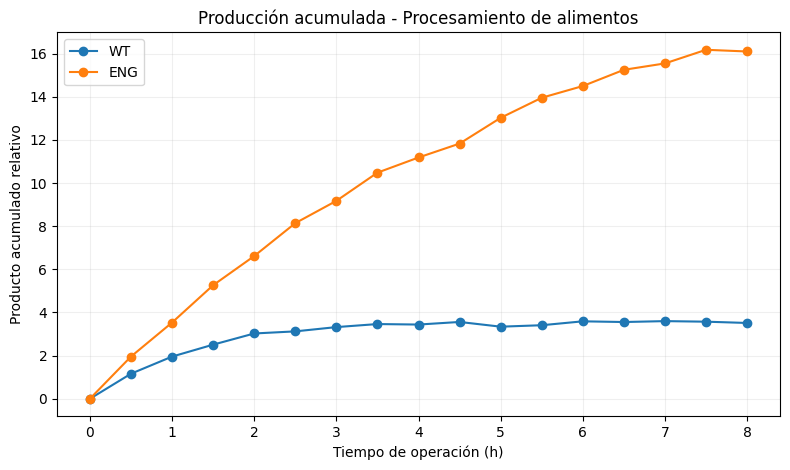
\includegraphics[width=0.43\textwidth]{13.png}
}
&
\parbox{0.46\textwidth}{
    \centering
    \small Caso 2: Bagazo de Caña\\[0.12cm]
    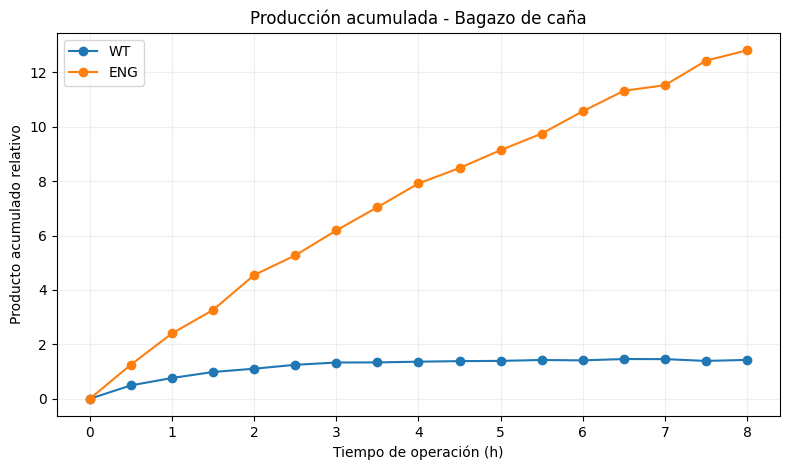
\includegraphics[width=0.43\textwidth]{14.png}
}
\\
\hline

\parbox{0.46\textwidth}{
    \centering
    \small Caso 3: Procesamiento de Biomasa\\[0.12cm]
    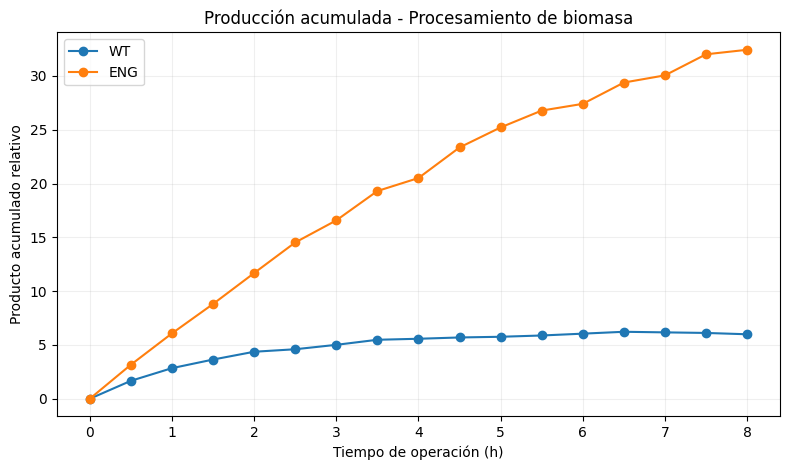
\includegraphics[width=0.43\textwidth]{15.png}
}
&
\parbox{0.46\textwidth}{
    \centering
    \small Caso 4: Síntesis de Glucósidos\\[0.12cm]
    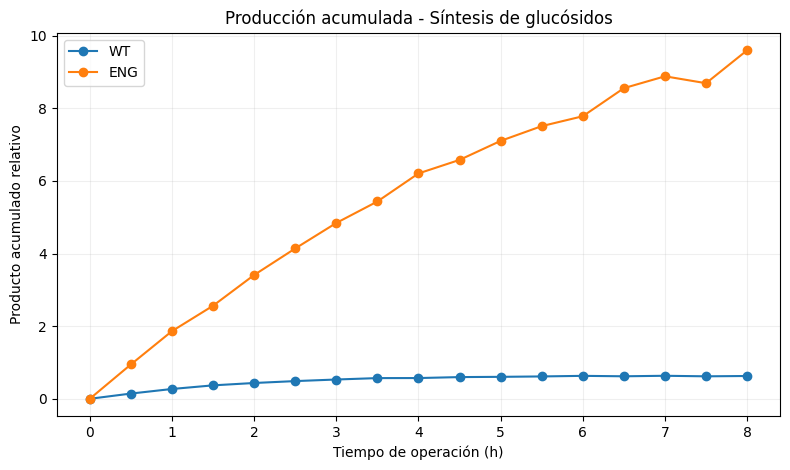
\includegraphics[width=0.43\textwidth]{16.png}
}
\\
\hline

\end{tabular}

\figcaptionlink{anx:fig_produccion}{Producción Acumulada Bajo la Condición Base}{fig:produccion_casos}


\end{figure}

\subsubsection{Caso 1: Procesamiento de Alimentos}

La proteasa ENG conserva actividad durante más tiempo que WT y alcanza
\(4.58\times\) la producción acumulada bajo la condición base. La principal
ganancia es extender la vida operativa sin sacrificar capacidad de conversión
\citep{yuan_apre2709_2025}. Las curvas completas de estabilidad se presentan en
el \anexolink{anx:estabilidad}{Estabilidad Térmica}.

\subsubsection{Caso 2: Bagazo de Caña}

La beta-glucosidasa ENG combina mayor estabilidad con mayor tolerancia a glucosa.
El producto acumulado alcanza \(8.96\times\) el valor de WT. En este caso, la
ventaja principal es mantener la reacción activa cuando el producto comienza a
inhibirla \citep{cao_ks5a7_2018}. La evidencia de estabilidad y cinética se
presenta en los \anexolink{anx:estabilidad}{Estabilidad Térmica} y \anexolink{anx:cinetica}{Cinética Frente a Concentración de Sustrato}.

\subsubsection{Caso 3: Procesamiento de Biomasa}

La xilanasa ENG desplaza su respuesta hacia temperaturas más elevadas y alcanza
\(5.41\times\) la producción de WT bajo la condición base
\citep{zhang_xylanase_2010}. La comparación térmica completa se presenta en el
\anexolink{anx:temperatura}{Respuesta Térmica}.

\subsubsection{Caso 4: Síntesis de Glucósidos}

La variante ENG combina estabilidad, mayor eficiencia y mejor selectividad. El
efecto conjunto genera el mayor aumento bajo condición base:
\(15.29\times\) la producción de WT \citep{yin_bgl1d_2019}. La cinética y la
selectividad se presentan en los \anexolink{anx:cinetica}{Cinética Frente a Concentración de Sustrato} y
\anexolink{anx:selectividad}{Selectividad en Síntesis de Glucósidos}.

\subsection{Resumen Cuantitativo}
\label{subsec:resumen_cuantitativo}

El Cuadro \ref{tab:resumen_resultados} concentra los resultados necesarios para
la decisión posterior.

\begin{table}[H]
\centering
\tabcaptionlink{anx:tab_resumen}{Resumen Cuantitativo Bajo la Condición Base}{tab:resumen_resultados}



\renewcommand{\arraystretch}{1.35}
\setlength{\tabcolsep}{3.5pt}

\begin{tabularx}{\textwidth}{
|p{2.5cm}|
>{\centering\arraybackslash}p{2.0cm}|
>{\centering\arraybackslash}p{1.45cm}|
>{\centering\arraybackslash}p{1.45cm}|
>{\centering\arraybackslash}p{1.45cm}|
>{\centering\arraybackslash}p{2.0cm}|
X|
}
\hline
Aplicación &
\(t_{50}\) WT \(\rightarrow\) ENG &
\(I_S\) &
\(I_C\) &
\(I_P\) &
\(T_{\mathrm{opt}}\) WT \(\rightarrow\) ENG &
Lectura \\ \hline

Alimentos &
1.11 \(\rightarrow\) 3.53 h &
3.37 &
1.54 &
4.58 &
60 \(\rightarrow\) 65 \(^{\circ}\)C &
La vida operativa impulsa el resultado. \\ \hline

Bagazo &
0.75 \(\rightarrow\) 7.02 h &
6.92 &
1.48 &
8.96 &
55 \(\rightarrow\) 65 \(^{\circ}\)C &
Estabilidad y tolerancia al producto. \\ \hline

Biomasa &
0.99 \(\rightarrow\) 6.13 h &
4.86 &
1.58 &
5.41 &
65 \(\rightarrow\) 75 \(^{\circ}\)C &
Mayor ventana térmica útil. \\ \hline

Glucósidos &
1.49 \(\rightarrow\) 5.43 h &
3.19 &
2.56 &
15.29 &
55 \(\rightarrow\) 60 \(^{\circ}\)C &
Eficiencia y selectividad amplifican la mejora. \\ \hline

\end{tabularx}
\end{table}

Los índices \(I_S\), \(I_C\) e \(I_P\) son mayores que 1 en los cuatro casos.
La mejora conjunta existe, pero su efecto sobre producción es distinto según el
mecanismo dominante.

\subsection{Comparación Gráfica}
\label{subsec:comparacion_grafica}

\begin{figure}[H]
\centering

\begin{tabular}{|c|c|}
\hline

\parbox{0.46\textwidth}{
    \centering
    \small (a) Impacto sobre Producción\\[0.12cm]
    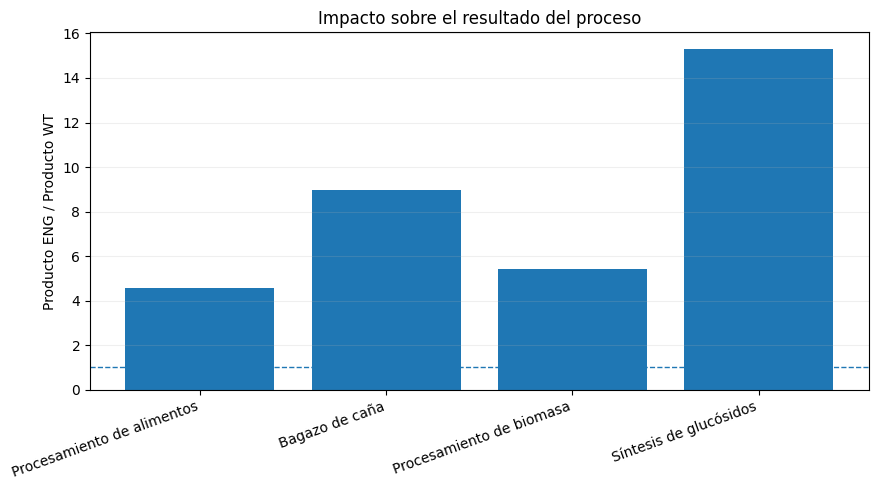
\includegraphics[width=0.43\textwidth]{20.png}
}
&
\parbox{0.46\textwidth}{
    \centering
    \small (b) Matriz Estabilidad--Eficiencia\\[0.12cm]
    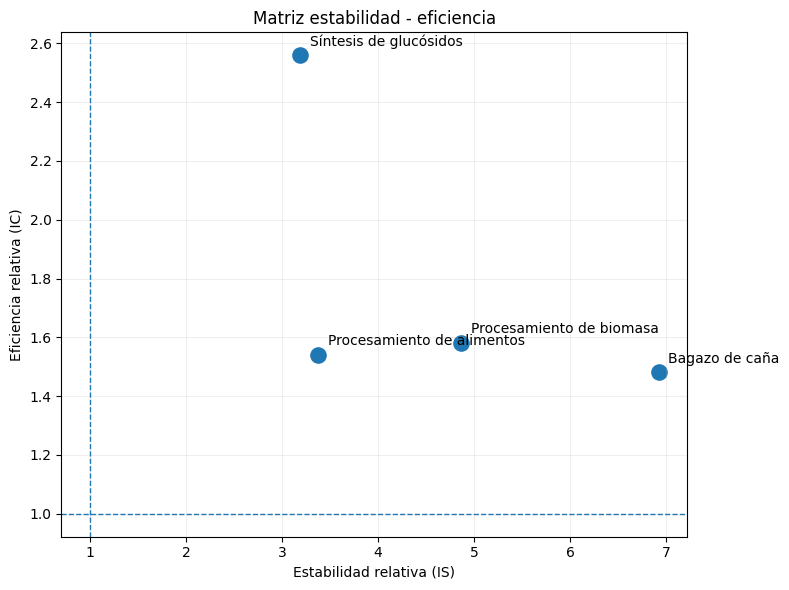
\includegraphics[width=0.43\textwidth]{21.png}
}
\\
\hline

\end{tabular}

\figcaptionlink{anx:fig_sintesis}{Síntesis Comparativa de los Cuatro Casos}{fig:resumen_experimento}


\end{figure}

La comparación individual de estabilidad y eficiencia se encuentra en el
\anexolink{anx:fig_sintesis}{Síntesis Comparativa de los Cuatro Casos}. No se repiten aquí esas figuras para mantener el cuerpo
principal orientado a resultados.

\subsection{Comportamientos que Limitan la Mejora}
\label{subsec:fenomenos}

La Figura \ref{fig:fenomenos} muestra por qué una mayor estabilidad o eficiencia
no se traduce siempre de forma proporcional en producto.

\begin{figure}[H]
\centering

\begin{tabular}{|c|c|}
\hline

\parbox{0.46\textwidth}{
    \centering
    \small (a) Proteasa: Riesgo de Inactivación\\[0.12cm]
    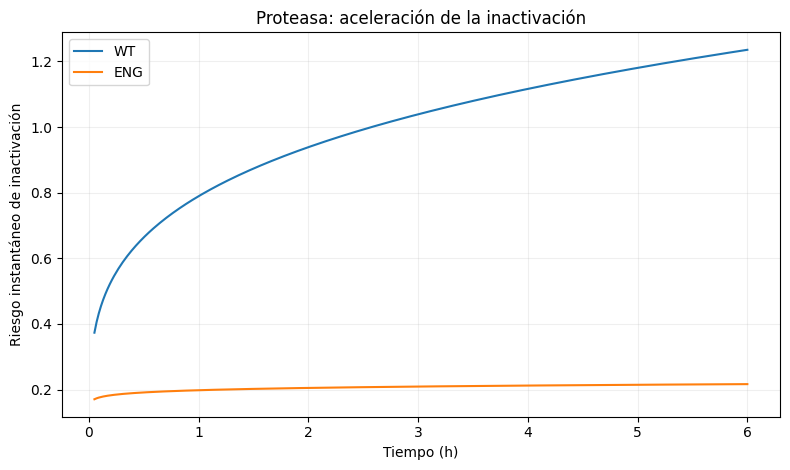
\includegraphics[width=0.43\textwidth]{22.png}
}
&
\parbox{0.46\textwidth}{
    \centering
    \small (b) Bagazo: Inhibición por Producto\\[0.12cm]
    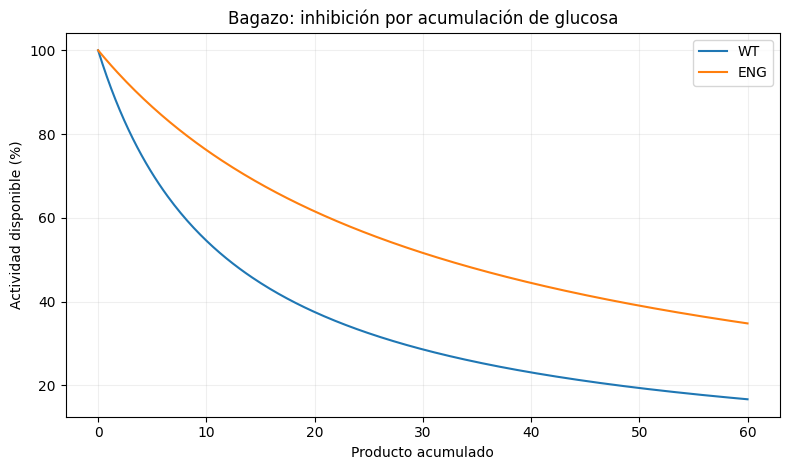
\includegraphics[width=0.43\textwidth]{23.png}
}
\\
\hline

\parbox{0.46\textwidth}{
    \centering
    \small (c) Biomasa: Activación Térmica Transitoria\\[0.12cm]
    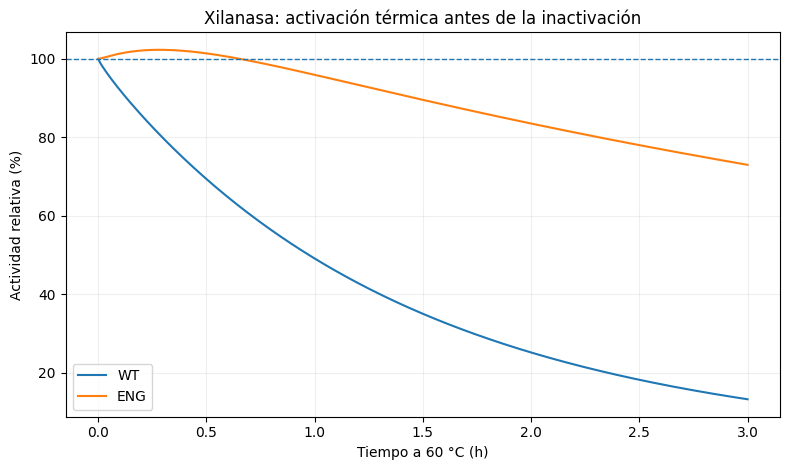
\includegraphics[width=0.43\textwidth]{24.png}
}
&
\parbox{0.46\textwidth}{
    \centering
    \small (d) Glucósidos: Inhibición por Sustrato\\[0.12cm]
    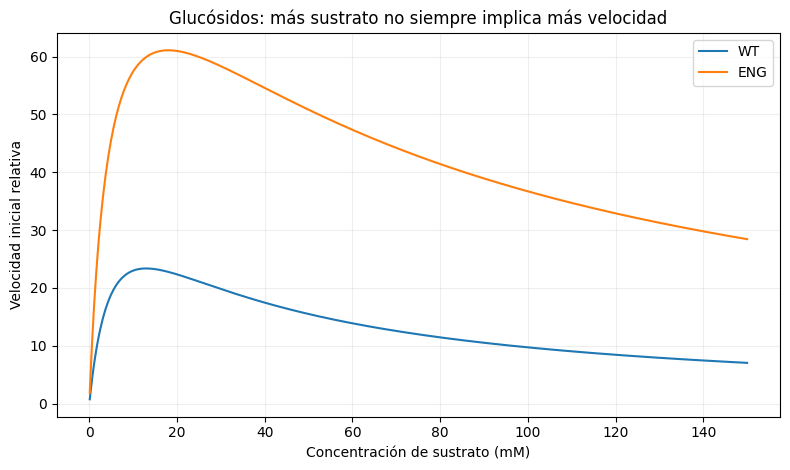
\includegraphics[width=0.43\textwidth]{25.png}
}
\\
\hline

\end{tabular}

\figcaptionlink{anx:fig_restricciones}{Restricciones No Lineales Observadas en los Cuatro Casos}{fig:fenomenos}


\end{figure}

\noindent\small
Evidencia complementaria:
\anexolink{anx:fig_restricciones}{Restricciones No Lineales Observadas en los Cuatro Casos} y
\anexolink{anx:selectividad}{Selectividad en Síntesis de Glucósidos}.
\normalsize

Los mecanismos son distintos: inactivación en alimentos, inhibición por producto
en bagazo, respuesta térmica en biomasa e inhibición por exceso de sustrato en
glucósidos. En este último caso, la selectividad introduce además una segunda
condición de decisión.

\subsection{Resultado General}
\label{subsec:resultado_general}

Los resultados responden la pregunta central: mejorar estabilidad no obligó a
sacrificar eficiencia en ninguno de los cuatro casos. Sin embargo, la mejora
molecular solo genera su máximo valor cuando se opera dentro de condiciones que
eviten el nuevo cuello de botella.

La \hyperref[sec:discusion]{Sección 5} transforma estos resultados en decisiones
concretas de operación y prioridad de explotación.

\section{Discusión y Explotación Industrial}
\label{sec:discusion}

Los resultados permiten pasar de una comparación bioquímica a una decisión
operativa. La pregunta ya no es solamente qué enzima es mejor, sino qué propiedad
genera valor en cada proceso y en qué condición conviene explotarla.

\subsection{Diagnóstico por Aplicación}
\label{subsec:diagnostico_industrial}

\begin{table}[H]
\centering
\tabcaptionlink{anx:tab_diagnostico}{Diagnóstico Industrial de los Cuatro Casos}{tab:diagnostico_industrial}



\renewcommand{\arraystretch}{1.3}

\begin{tabularx}{\textwidth}{
|p{2.4cm}|
p{3.2cm}|
p{3.2cm}|
X|
}
\hline
Aplicación & Cuello de botella observado & Evidencia principal & Acción prioritaria \\ \hline

Alimentos &
Inactivación temprana &
\(t_{50}\): 1.11 \(\rightarrow\) 3.53 h &
Explotar mayor vida operativa antes de buscar más velocidad. \\ \hline

Bagazo &
Inactivación e inhibición por glucosa &
\(t_{50}\): 0.75 \(\rightarrow\) 7.02 h &
Priorizar estabilidad y tolerancia al producto. \\ \hline

Biomasa &
Ventana térmica &
\(T_{\mathrm{opt}}\): 65 \(\rightarrow\) 75 \(^{\circ}\)C &
Aprovechar temperaturas mayores sin exceder el punto productivo. \\ \hline

Glucósidos &
Inhibición y selectividad &
\(I_C=2.56\), \(I_P=15.29\) &
Optimizar producto útil, no velocidad aislada. \\ \hline

\end{tabularx}
\end{table}

La evidencia gráfica que respalda estos diagnósticos se encuentra en el
\anexolink{anx:estabilidad}{Estabilidad Térmica}, el
\anexolink{anx:temperatura}{Respuesta Térmica} y el
\anexolink{anx:selectividad}{Selectividad en Síntesis de Glucósidos}.

\subsection{Cuánto de la Mejora Llega a Producción}
\label{subsec:traduccion_produccion}

El factor de traducción productiva \(F_P\), definido en la Sección
\ref{subsec:indicadores}, permite distinguir entre mejora molecular y mejora de
proceso.

\begin{table}[H]
\centering
\tabcaptionlink{anx:tab_traduccion}{Traducción de la Mejora Molecular a Producción}{tab:factor_traduccion}



\renewcommand{\arraystretch}{1.25}

\begin{tabular}{|l|c|l|}
\hline
Aplicación & \(F_P\) & Lectura \\ \hline
Alimentos & 0.88 & Ligera atenuación por restricciones del proceso. \\ \hline
Bagazo de caña & 0.87 & La inhibición absorbe parte de la mejora. \\ \hline
Biomasa & 0.70 & La estabilidad deja de ser el único límite. \\ \hline
Glucósidos & 1.87 & Selectividad y tolerancia amplifican el resultado. \\ \hline
\end{tabular}
\end{table}

Biomasa y glucósidos muestran el contraste más útil. En biomasa, continuar
invirtiendo únicamente en estabilidad ofrece retornos técnicos decrecientes. En
glucósidos, propiedades adicionales amplifican la mejora de estabilidad y
eficiencia.

\subsection{Puntos de Operación para Capturar Valor}
\label{subsec:monetizacion}

Para esta etapa se comparó el mejor punto encontrado para ENG con el mejor punto
encontrado para WT dentro de la misma malla evaluada: \(35--90\,^{\circ}\mathrm{C}\),
0.5--80 mM de sustrato y ocho horas de operación.

Esta comparación es distinta de \(I_P\): \(I_P\) usa una condición base común;
el Cuadro \ref{tab:puntos_operacion} permite que cada variante opere en su mejor
punto dentro del rango analizado.

\begin{table}[H]
\centering
\tabcaptionlink{anx:tab_puntos}{Puntos de Operación con Mayor Producto Dentro del Rango Evaluado}{tab:puntos_operacion}



\renewcommand{\arraystretch}{1.35}
\setlength{\tabcolsep}{3.5pt}

\begin{tabularx}{\textwidth}{
|p{2.1cm}|
>{\centering\arraybackslash}p{2.0cm}|
>{\centering\arraybackslash}p{1.5cm}|
>{\centering\arraybackslash}p{2.0cm}|
>{\centering\arraybackslash}p{1.5cm}|
>{\centering\arraybackslash}p{1.5cm}|
X|
}
\hline
Aplicación &
ENG: \(T\), sustrato &
Producto ENG &
WT: \(T\), sustrato &
Producto WT &
Ventaja &
Decisión \\ \hline

Alimentos &
60 \(^{\circ}\)C, 40 mM &
16.47 &
45 \(^{\circ}\)C, 40 mM &
5.93 &
2.78\(\times\) &
Usar ENG para extender producción. \\ \hline

Bagazo &
60 \(^{\circ}\)C, 40 mM &
12.70 &
45 \(^{\circ}\)C, 20 mM &
2.93 &
4.33\(\times\) &
Explotar estabilidad y tolerancia a glucosa. \\ \hline

Biomasa &
70 \(^{\circ}\)C, 80 mM &
36.04 &
50 \(^{\circ}\)C, 40 mM &
7.38 &
4.88\(\times\) &
Operar ENG a mayor temperatura y carga. \\ \hline

Glucósidos &
60 \(^{\circ}\)C, 40 mM &
9.49 &
45 \(^{\circ}\)C, 20 mM &
1.59 &
5.95\(\times\) &
Priorizar producto útil y selectividad. \\ \hline

\end{tabularx}
\end{table}

\subsubsection{A. Alimentos}

La recomendación es operar ENG a \(60\,^{\circ}\mathrm{C}\), 40 mM y ocho horas.
Dentro del rango evaluado produce \(2.78\times\) el mejor resultado de WT, es
decir, aproximadamente 178\% más producto.

La razón es la duración: ENG mantiene actividad durante más tiempo. No conviene
elegir automáticamente \(65\,^{\circ}\mathrm{C}\) por ser la temperatura de
máxima actividad instantánea; el mejor resultado acumulado aparece a
\(60\,^{\circ}\mathrm{C}\).

\subsubsection{B. Bagazo de Caña}

La recomendación es ENG a \(60\,^{\circ}\mathrm{C}\), 40 mM y ocho horas.
La ventaja frente al mejor punto de WT es \(4.33\times\), aproximadamente
333\% más producto.

La prioridad no es aumentar otra vez la velocidad inicial. El valor proviene de
mantener la enzima activa y reducir el efecto de la glucosa acumulada.

\subsubsection{C. Biomasa}

La mejor condición encontrada para ENG es aproximadamente
\(70\,^{\circ}\mathrm{C}\) y 80 mM. El producto alcanza 36.04 unidades relativas,
frente a 7.38 del mejor punto de WT: \(4.88\times\), aproximadamente 388\% más.

La temperatura de máxima actividad instantánea de ENG es
\(75\,^{\circ}\mathrm{C}\), pero el mayor producto acumulado aparece a
\(70\,^{\circ}\mathrm{C}\). Para operación industrial debe priorizarse el segundo
criterio.

\subsubsection{D. Glucósidos}

La recomendación es ENG a \(60\,^{\circ}\mathrm{C}\), 40 mM y ocho horas.
La ventaja frente al mejor punto de WT es \(5.95\times\), aproximadamente
495\% más producto útil.

No conviene aumentar sustrato indefinidamente. La decisión debe equilibrar
inhibición y selectividad, utilizando como objetivo final la cantidad de
glucósido deseado.

\subsection{Prioridad de Explotación}
\label{subsec:prioridad_inversion}

Si el criterio es únicamente el aumento relativo de producto dentro del rango
evaluado, la prioridad es:

\begin{enumerate}
    \item síntesis de glucósidos: \(5.95\times\), aproximadamente \(+495\%\);
    \item procesamiento de biomasa: \(4.88\times\), aproximadamente \(+388\%\);
    \item bagazo de caña: \(4.33\times\), aproximadamente \(+333\%\);
    \item procesamiento de alimentos: \(2.78\times\), aproximadamente \(+178\%\).
\end{enumerate}

Este orden no representa rentabilidad neta. Representa potencial productivo. Para
convertirlo en margen económico real faltan solo tres datos específicos de cada
planta: precio del producto útil, costo de ENG frente a WT y costo energético de
la condición de operación.

La decisión técnica, sin embargo, ya es concreta: glucósidos ofrece la mayor
ventaja relativa; biomasa exige explotar la ventana térmica; bagazo exige
estabilidad y tolerancia; alimentos exige vida operativa.

\section{Conclusiones}
\label{sec:conclusiones}

Los resultados permiten responder directamente la pregunta planteada:

\begin{enumerate}

    \item Mejorar termoestabilidad no obligó a sacrificar eficiencia. En los
    cuatro casos se obtuvo \(I_S>1\) e \(I_C>1\).

    \item Bajo la condición base común, ENG generó entre \(4.58\times\) y
    \(15.29\times\) la producción de WT. La magnitud depende del cuello de
    botella de cada aplicación.

    \item Cuando cada variante se llevó a su mejor punto dentro del rango
    evaluado, ENG mantuvo una ventaja de \(2.78\times\) a \(5.95\times\).
    Por tanto, la ventaja no depende únicamente de haber elegido una condición
    desfavorable para WT.

    \item El punto de máxima actividad no siempre coincide con el de máxima
    producción. Biomasa lo muestra con claridad: ENG presenta máxima actividad
    alrededor de \(75\,^{\circ}\mathrm{C}\), pero su mayor producto acumulado
    aparece alrededor de \(70\,^{\circ}\mathrm{C}\).

    \item La decisión industrial debe atacar el cuello de botella concreto:
    vida operativa en alimentos, estabilidad y tolerancia en bagazo, ventana
    térmica en biomasa y selectividad en glucósidos.
\end{enumerate}

La conclusión general es:

\begin{equation}
\text{Ingeniería Enzimática}
\longrightarrow
\text{Mejora Molecular}
\longrightarrow
\text{Control del Cuello de Botella}
\longrightarrow
\text{Mayor Producción Útil}.
\end{equation}

La ingeniería enzimática puede mejorar simultáneamente estabilidad y eficiencia,
pero su valor industrial depende de operar la variante en condiciones que
conviertan esa mejora en producto
\citep{siddiqui_defying_2017,hou_tradeoff_2023}.


% 14. referencias
\clearpage
\bibliographystyle{apacite}
\bibliography{referencias}

% 15. anexos
\clearpage
\appendix

\renewcommand{\thefigure}{\thesection.\arabic{figure}}
\renewcommand{\thetable}{\thesection.\arabic{table}}
\renewcommand{\theequation}{\thesection.\arabic{equation}}

\section{Correspondencia de Figuras y Cuadros}
\label{sec:anexos}

\subsection{Relación entre las Variables del Análisis}
\label{anx:fig_variables}

\begin{equation}
\text{Estabilidad}
+
\text{Eficiencia}
+
\text{Condiciones de Operación}
\longrightarrow
\text{Producción Útil}.
\end{equation}

\begin{center}
\small\hyperref[fig:variables]{Volver a la Figura \ref*{fig:variables}}
\end{center}


\subsection{Protocolo Utilizado para Comparar WT y ENG}
\label{anx:tab_protocolo}

\begin{table}[H]
\centering
\caption{Protocolo Utilizado para Comparar WT y ENG}
\caption*{\small\textit{Fuente:} Elaboración propia.}
\renewcommand{\arraystretch}{1.25}
\begin{tabularx}{0.96\textwidth}{|p{2.6cm}|p{4.1cm}|X|}
\hline
Prueba & Condición & Resultado Utilizado \\ \hline
Estabilidad & \(60\,^{\circ}\mathrm{C}\), 10 mM de sustrato &
\(t_{50}\) y actividad conservada en el tiempo. \\ \hline
Cinética & 0.5--80 mM de sustrato &
Eficiencia de conversión e inhibición por exceso de sustrato. \\ \hline
Respuesta Térmica & \(35--90\,^{\circ}\mathrm{C}\) &
Temperatura de máxima actividad. \\ \hline
Producción Base & \(60\,^{\circ}\mathrm{C}\), 40 mM, 8 horas &
Producto acumulado bajo una condición común. \\ \hline
Exploración Operativa & Misma malla de temperaturas y sustratos, 8 horas &
Mejor punto de producción encontrado para WT y ENG. \\ \hline
\end{tabularx}
\end{table}

\begin{center}
\small\hyperref[tab:protocolo_metodologia]{Volver al Cuadro \ref*{tab:protocolo_metodologia}}
\end{center}


\subsection{Lectura de los Índices}
\label{anx:tab_lectura_indices}

\begin{table}[H]
\centering
\caption{Lectura de los Índices}
\caption*{\small\textit{Fuente:} Elaboración propia.}
\renewcommand{\arraystretch}{1.25}
\begin{tabular}{|c|p{9.5cm}|}
\hline
Valor & Interpretación \\ \hline
\(>1\) & ENG mejora el resultado frente a WT. \\ \hline
\(=1\) & No existe diferencia entre ambas variantes. \\ \hline
\(<1\) & ENG obtiene un resultado inferior a WT. \\ \hline
\end{tabular}
\end{table}

\begin{center}
\small\hyperref[tab:lectura_indices]{Volver al Cuadro \ref*{tab:lectura_indices}}
\end{center}


\subsection{Flujo Metodológico Orientado a Decisión}
\label{anx:fig_flujo}

\begin{equation}
\text{Comparar WT--ENG}
\longrightarrow
\text{Medir}
\longrightarrow
\text{Identificar el Límite}
\longrightarrow
\text{Elegir el Punto Operativo}.
\end{equation}

\begin{center}
\small\hyperref[fig:flujo_metodologia]{Volver a la Figura \ref*{fig:flujo_metodologia}}
\end{center}


\subsection{Producción Acumulada Bajo la Condición Base}
\label{anx:fig_produccion}

\begin{figure}[H]
\centering
\begin{tabular}{|c|c|}
\hline
\parbox{0.46\textwidth}{\centering\small Caso 1: Procesamiento de Alimentos\\[0.12cm]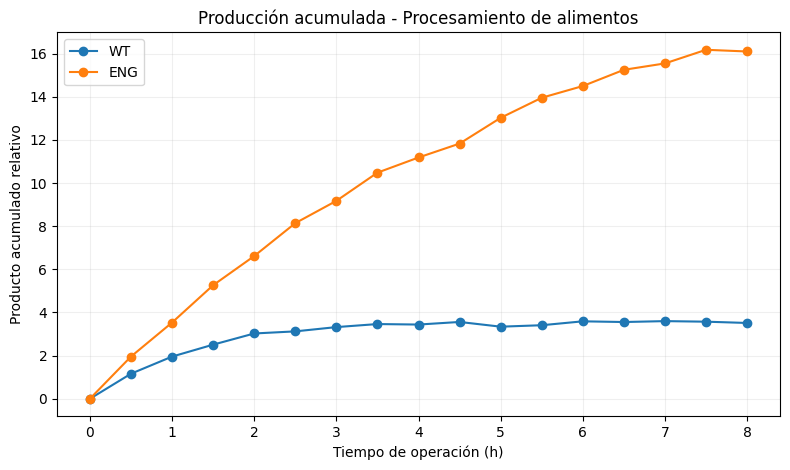
\includegraphics[width=0.43\textwidth]{13.png}}
&
\parbox{0.46\textwidth}{\centering\small Caso 2: Bagazo de Caña\\[0.12cm]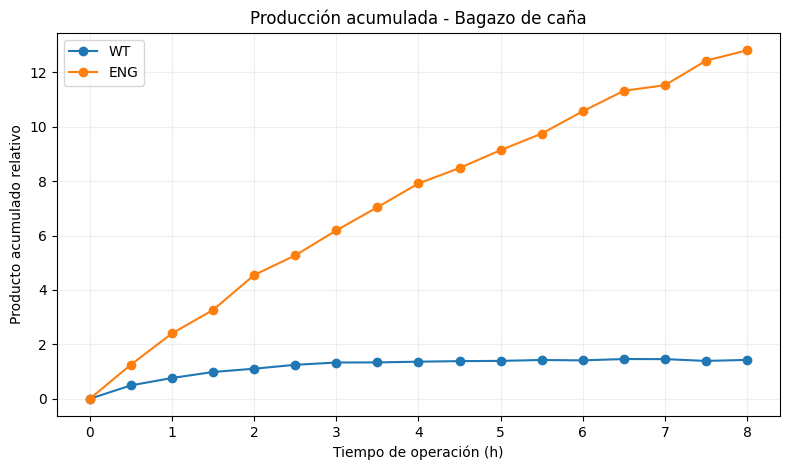
\includegraphics[width=0.43\textwidth]{14.png}}
\\ \hline
\parbox{0.46\textwidth}{\centering\small Caso 3: Procesamiento de Biomasa\\[0.12cm]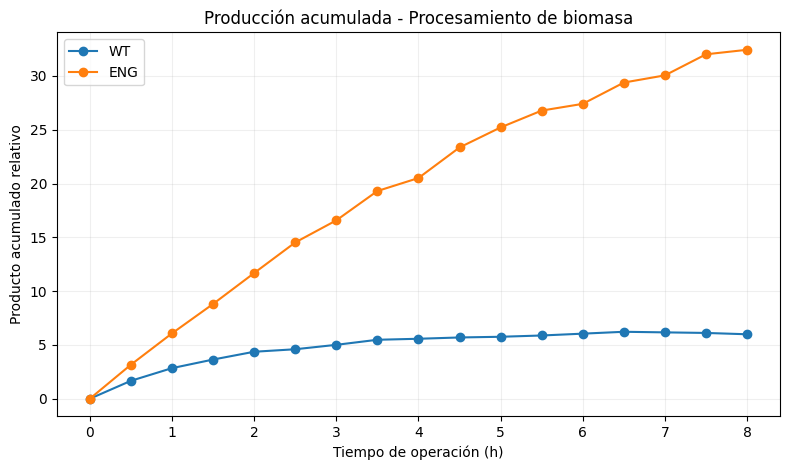
\includegraphics[width=0.43\textwidth]{15.png}}
&
\parbox{0.46\textwidth}{\centering\small Caso 4: Síntesis de Glucósidos\\[0.12cm]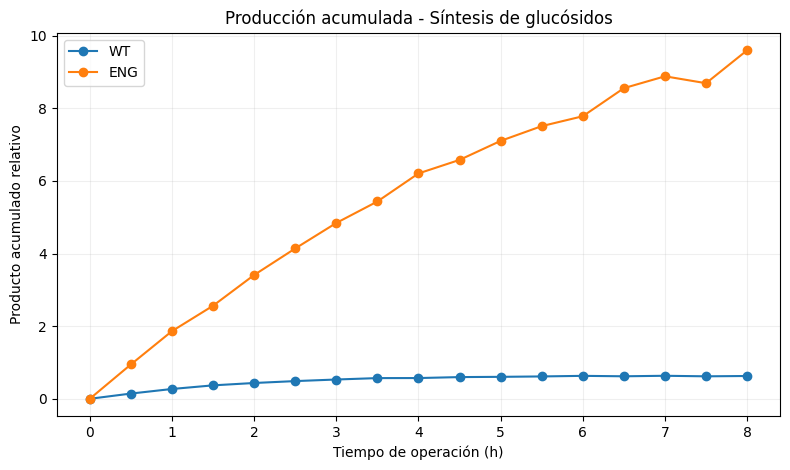
\includegraphics[width=0.43\textwidth]{16.png}}
\\ \hline
\end{tabular}
\caption{Producción Acumulada Bajo la Condición Base}
\caption*{\small\textit{Fuente:} Elaboración propia.}
\end{figure}

\begin{center}
\small\hyperref[fig:produccion_casos]{Volver a la Figura \ref*{fig:produccion_casos}}
\end{center}


\subsection{Resumen Cuantitativo Bajo la Condición Base}
\label{anx:tab_resumen}

\begin{table}[H]
\centering
\caption{Resumen Cuantitativo Bajo la Condición Base}
\caption*{\small\textit{Fuente:} Elaboración propia.}
\renewcommand{\arraystretch}{1.25}
\setlength{\tabcolsep}{3.5pt}
\begin{tabularx}{\textwidth}{
|p{2.5cm}|
>{\centering\arraybackslash}p{2.0cm}|
>{\centering\arraybackslash}p{1.45cm}|
>{\centering\arraybackslash}p{1.45cm}|
>{\centering\arraybackslash}p{1.45cm}|
>{\centering\arraybackslash}p{2.0cm}|
X|}
\hline
Aplicación & \(t_{50}\) WT \(\rightarrow\) ENG & \(I_S\) & \(I_C\) & \(I_P\) &
\(T_{\mathrm{opt}}\) WT \(\rightarrow\) ENG & Lectura \\ \hline
Alimentos & 1.11 \(\rightarrow\) 3.53 h & 3.37 & 1.54 & 4.58 &
60 \(\rightarrow\) 65 \(^{\circ}\)C & La vida operativa impulsa el resultado. \\ \hline
Bagazo & 0.75 \(\rightarrow\) 7.02 h & 6.92 & 1.48 & 8.96 &
55 \(\rightarrow\) 65 \(^{\circ}\)C & Estabilidad y tolerancia al producto. \\ \hline
Biomasa & 0.99 \(\rightarrow\) 6.13 h & 4.86 & 1.58 & 5.41 &
65 \(\rightarrow\) 75 \(^{\circ}\)C & Mayor ventana térmica útil. \\ \hline
Glucósidos & 1.49 \(\rightarrow\) 5.43 h & 3.19 & 2.56 & 15.29 &
55 \(\rightarrow\) 60 \(^{\circ}\)C & Eficiencia y selectividad amplifican la mejora. \\ \hline
\end{tabularx}
\end{table}

\begin{center}
\small\hyperref[tab:resumen_resultados]{Volver al Cuadro \ref*{tab:resumen_resultados}}
\end{center}


\subsection{Síntesis Comparativa de los Cuatro Casos}
\label{anx:fig_sintesis}

\begin{figure}[H]
\centering
\begin{tabular}{|c|c|}
\hline
\parbox{0.46\textwidth}{\centering\small Impacto sobre Producción\\[0.12cm]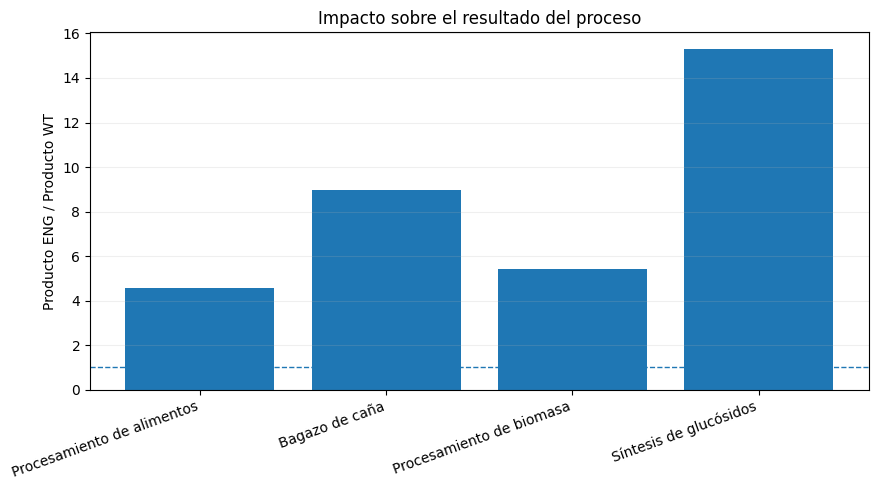
\includegraphics[width=0.43\textwidth]{20.png}}
&
\parbox{0.46\textwidth}{\centering\small Matriz Estabilidad--Eficiencia\\[0.12cm]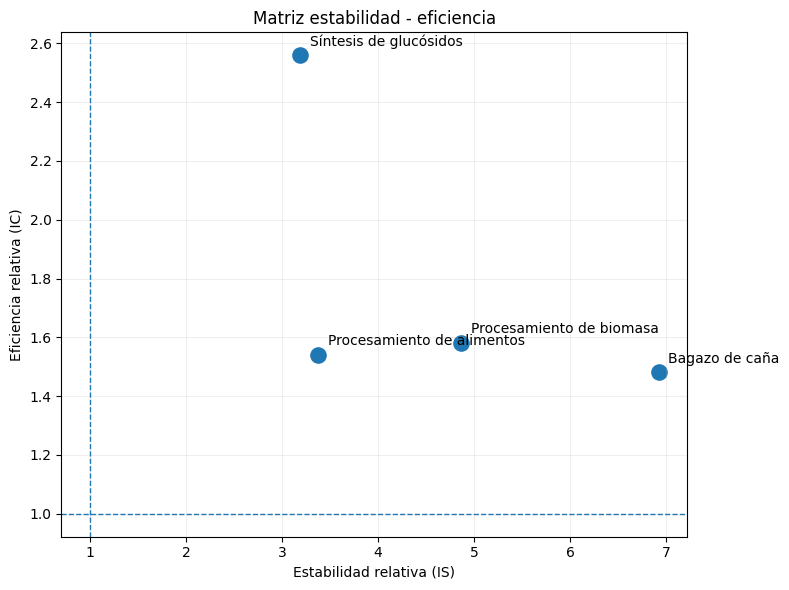
\includegraphics[width=0.43\textwidth]{21.png}}
\\ \hline
\end{tabular}
\caption{Síntesis Comparativa de los Cuatro Casos}
\caption*{\small\textit{Fuente:} Elaboración propia.}
\end{figure}

\begin{center}
\small\hyperref[fig:resumen_experimento]{Volver a la Figura \ref*{fig:resumen_experimento}}
\end{center}


\subsection{Restricciones No Lineales Observadas en los Cuatro Casos}
\label{anx:fig_restricciones}
\label{anx:fenomenos}

\begin{figure}[H]
\centering
\begin{tabular}{|c|c|}
\hline
\parbox{0.46\textwidth}{\centering\small Proteasa: Riesgo de Inactivación\\[0.12cm]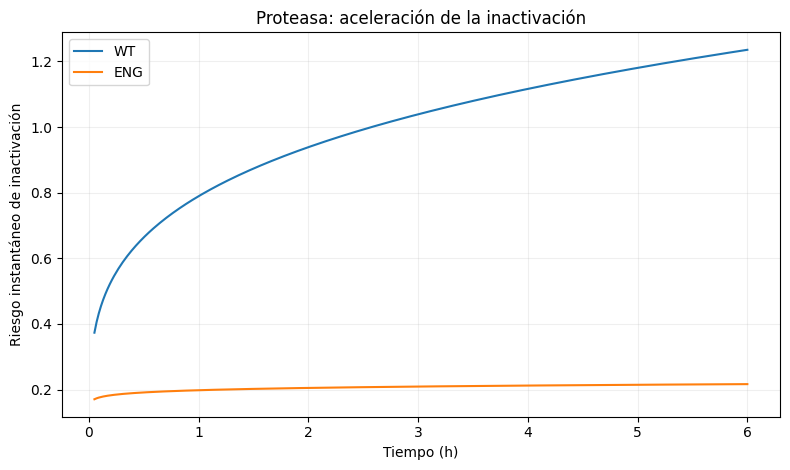
\includegraphics[width=0.43\textwidth]{22.png}}
&
\parbox{0.46\textwidth}{\centering\small Bagazo: Inhibición por Producto\\[0.12cm]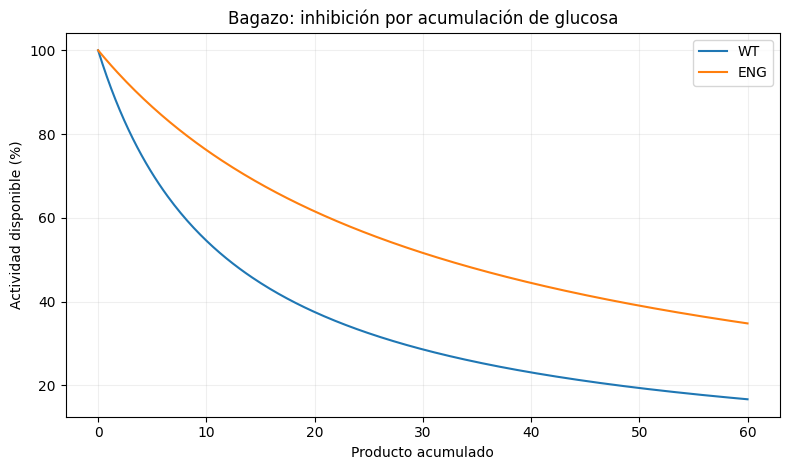
\includegraphics[width=0.43\textwidth]{23.png}}
\\ \hline
\parbox{0.46\textwidth}{\centering\small Biomasa: Activación Térmica Transitoria\\[0.12cm]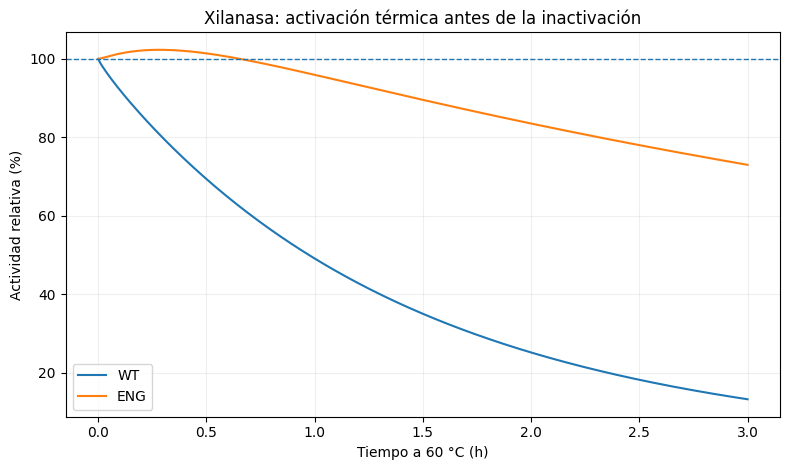
\includegraphics[width=0.43\textwidth]{24.png}}
&
\parbox{0.46\textwidth}{\centering\small Glucósidos: Inhibición por Sustrato\\[0.12cm]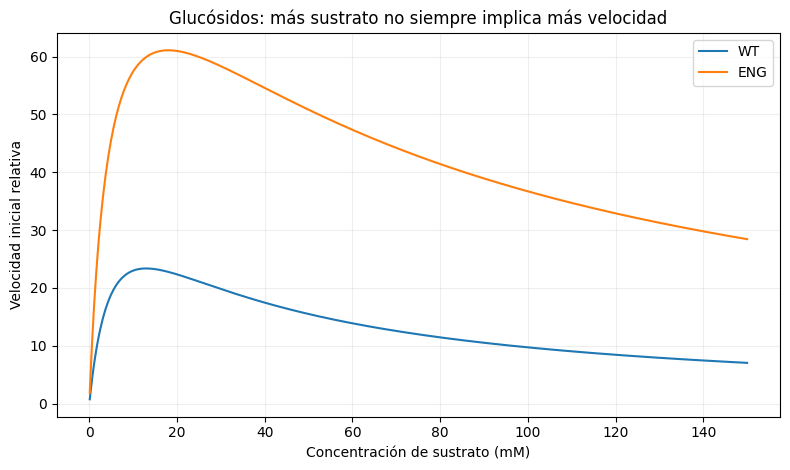
\includegraphics[width=0.43\textwidth]{25.png}}
\\ \hline
\end{tabular}
\caption{Restricciones No Lineales Observadas en los Cuatro Casos}
\caption*{\small\textit{Fuente:} Elaboración propia.}
\end{figure}

\begin{center}
\small\hyperref[fig:fenomenos]{Volver a la Figura \ref*{fig:fenomenos}}
\end{center}


\subsection{Diagnóstico Industrial de los Cuatro Casos}
\label{anx:tab_diagnostico}

\begin{table}[H]
\centering
\caption{Diagnóstico Industrial de los Cuatro Casos}
\caption*{\small\textit{Fuente:} Elaboración propia.}
\renewcommand{\arraystretch}{1.25}
\begin{tabularx}{\textwidth}{|p{2.4cm}|p{3.2cm}|p{3.2cm}|X|}
\hline
Aplicación & Cuello de Botella & Evidencia Principal & Acción Prioritaria \\ \hline
Alimentos & Inactivación temprana & \(t_{50}\): 1.11 \(\rightarrow\) 3.53 h &
Explotar mayor vida operativa. \\ \hline
Bagazo & Inactivación e inhibición por glucosa &
\(t_{50}\): 0.75 \(\rightarrow\) 7.02 h & Priorizar estabilidad y tolerancia. \\ \hline
Biomasa & Ventana térmica &
\(T_{\mathrm{opt}}\): 65 \(\rightarrow\) 75 \(^{\circ}\)C &
Aprovechar temperaturas mayores. \\ \hline
Glucósidos & Inhibición y selectividad &
\(I_C=2.56\), \(I_P=15.29\) & Optimizar producto útil. \\ \hline
\end{tabularx}
\end{table}

\begin{center}
\small\hyperref[tab:diagnostico_industrial]{Volver al Cuadro \ref*{tab:diagnostico_industrial}}
\end{center}


\subsection{Traducción de la Mejora Molecular a Producción}
\label{anx:tab_traduccion}

\begin{table}[H]
\centering
\caption{Traducción de la Mejora Molecular a Producción}
\caption*{\small\textit{Fuente:} Elaboración propia.}
\renewcommand{\arraystretch}{1.25}
\begin{tabular}{|l|c|l|}
\hline
Aplicación & \(F_P\) & Lectura \\ \hline
Alimentos & 0.88 & Ligera atenuación por restricciones del proceso. \\ \hline
Bagazo de Caña & 0.87 & La inhibición absorbe parte de la mejora. \\ \hline
Biomasa & 0.70 & La estabilidad deja de ser el único límite. \\ \hline
Glucósidos & 1.87 & Selectividad y tolerancia amplifican el resultado. \\ \hline
\end{tabular}
\end{table}

\begin{center}
\small\hyperref[tab:factor_traduccion]{Volver al Cuadro \ref*{tab:factor_traduccion}}
\end{center}


\subsection{Puntos de Operación con Mayor Producto Dentro del Rango Evaluado}
\label{anx:tab_puntos}

\begin{table}[H]
\centering
\caption{Puntos de Operación con Mayor Producto Dentro del Rango Evaluado}
\caption*{\small\textit{Fuente:} Elaboración propia.}
\renewcommand{\arraystretch}{1.25}
\setlength{\tabcolsep}{3.5pt}
\begin{tabularx}{\textwidth}{
|p{2.1cm}|
>{\centering\arraybackslash}p{2.0cm}|
>{\centering\arraybackslash}p{1.5cm}|
>{\centering\arraybackslash}p{2.0cm}|
>{\centering\arraybackslash}p{1.5cm}|
>{\centering\arraybackslash}p{1.5cm}|
X|}
\hline
Aplicación & ENG: \(T\), Sustrato & Producto ENG &
WT: \(T\), Sustrato & Producto WT & Ventaja & Decisión \\ \hline
Alimentos & 60 \(^{\circ}\)C, 40 mM & 16.47 &
45 \(^{\circ}\)C, 40 mM & 5.93 & 2.78\(\times\) &
Usar ENG para extender producción. \\ \hline
Bagazo & 60 \(^{\circ}\)C, 40 mM & 12.70 &
45 \(^{\circ}\)C, 20 mM & 2.93 & 4.33\(\times\) &
Explotar estabilidad y tolerancia a glucosa. \\ \hline
Biomasa & 70 \(^{\circ}\)C, 80 mM & 36.04 &
50 \(^{\circ}\)C, 40 mM & 7.38 & 4.88\(\times\) &
Operar ENG a mayor temperatura y carga. \\ \hline
Glucósidos & 60 \(^{\circ}\)C, 40 mM & 9.49 &
45 \(^{\circ}\)C, 20 mM & 1.59 & 5.95\(\times\) &
Priorizar producto útil y selectividad. \\ \hline
\end{tabularx}
\end{table}

\begin{center}
\small\hyperref[tab:puntos_operacion]{Volver al Cuadro \ref*{tab:puntos_operacion}}
\end{center}


\section{Evidencia Gráfica Complementaria}
\label{sec:evidencia_complementaria}

\subsection{Estabilidad Térmica}
\label{anx:estabilidad}

\begin{figure}[H]
\centering
\begin{tabular}{|c|c|}
\hline
\parbox{0.46\textwidth}{\centering\small Procesamiento de Alimentos\\[0.12cm]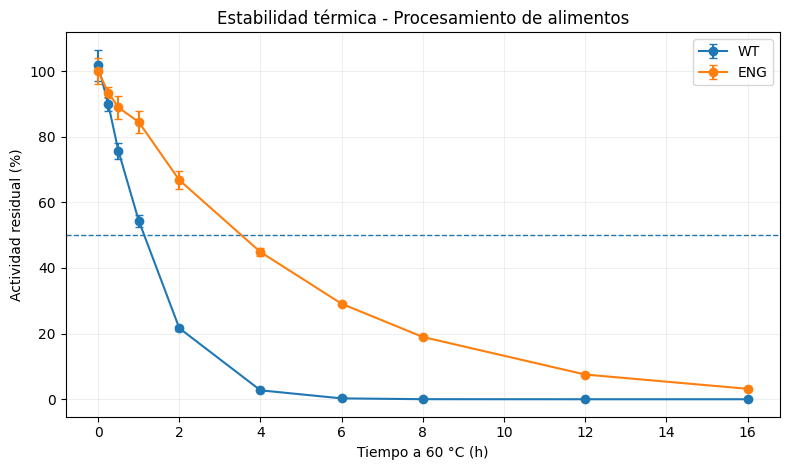
\includegraphics[width=0.43\textwidth]{1.png}}
&
\parbox{0.46\textwidth}{\centering\small Bagazo de Caña\\[0.12cm]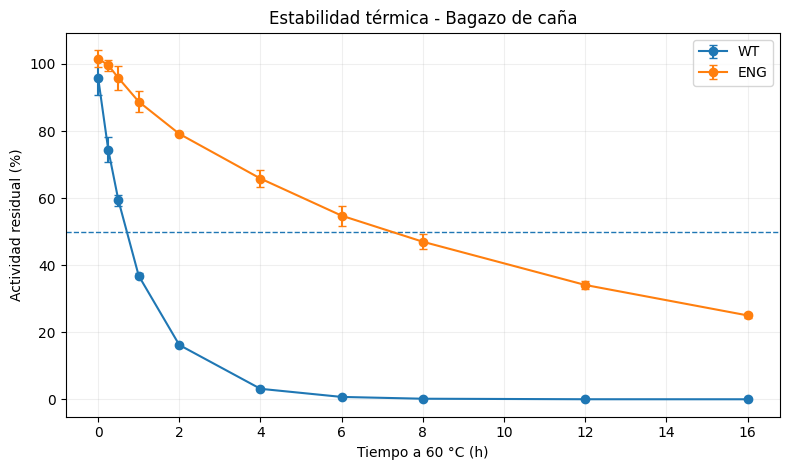
\includegraphics[width=0.43\textwidth]{2.png}}
\\ \hline
\parbox{0.46\textwidth}{\centering\small Procesamiento de Biomasa\\[0.12cm]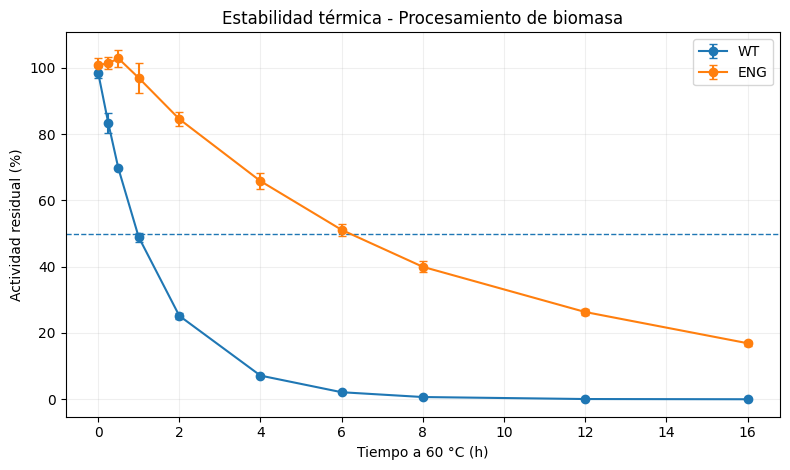
\includegraphics[width=0.43\textwidth]{3.png}}
&
\parbox{0.46\textwidth}{\centering\small Síntesis de Glucósidos\\[0.12cm]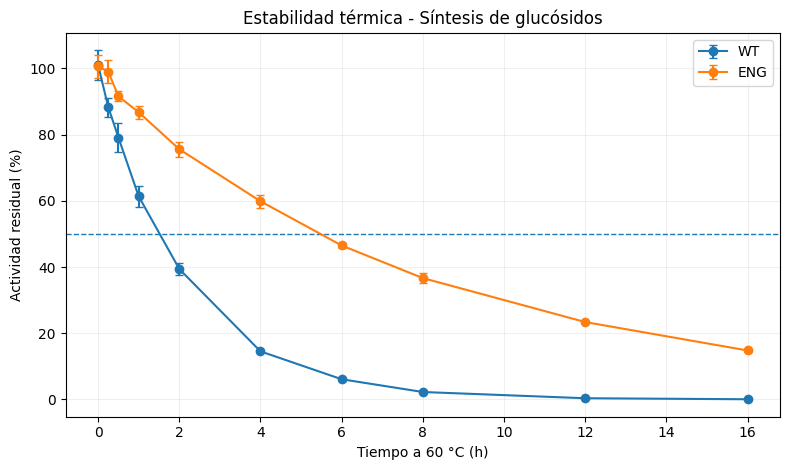
\includegraphics[width=0.43\textwidth]{4.png}}
\\ \hline
\end{tabular}
\caption{Estabilidad Térmica}
\caption*{\small\textit{Fuente:} Elaboración propia.}
\end{figure}


\subsection{Cinética Frente a Concentración de Sustrato}
\label{anx:cinetica}

\begin{figure}[H]
\centering
\begin{tabular}{|c|c|}
\hline
\parbox{0.46\textwidth}{\centering\small Procesamiento de Alimentos\\[0.12cm]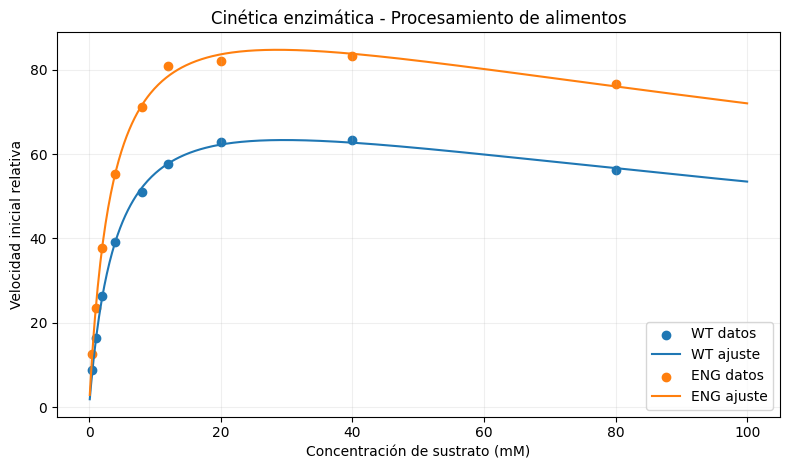
\includegraphics[width=0.43\textwidth]{5.png}}
&
\parbox{0.46\textwidth}{\centering\small Bagazo de Caña\\[0.12cm]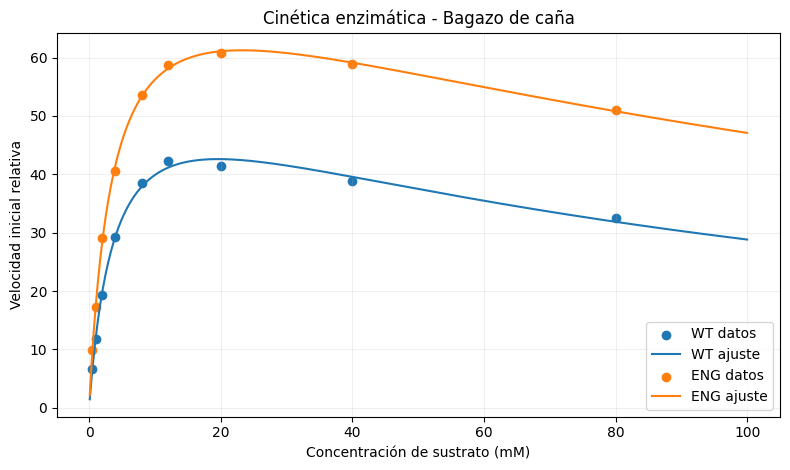
\includegraphics[width=0.43\textwidth]{6.png}}
\\ \hline
\parbox{0.46\textwidth}{\centering\small Procesamiento de Biomasa\\[0.12cm]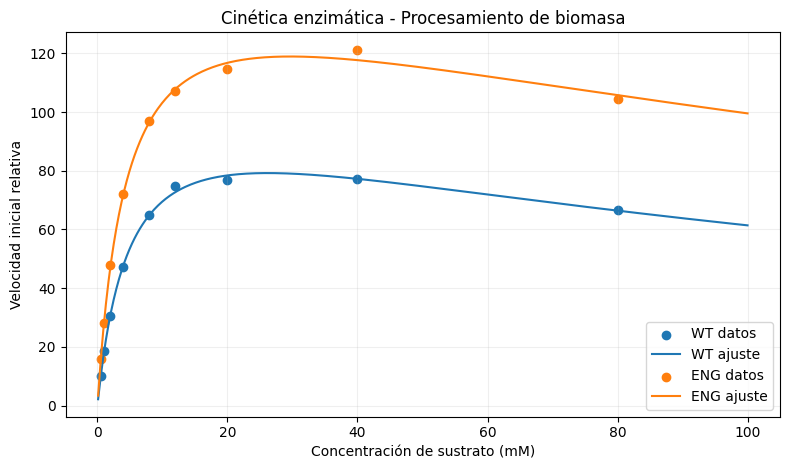
\includegraphics[width=0.43\textwidth]{7.png}}
&
\parbox{0.46\textwidth}{\centering\small Síntesis de Glucósidos\\[0.12cm]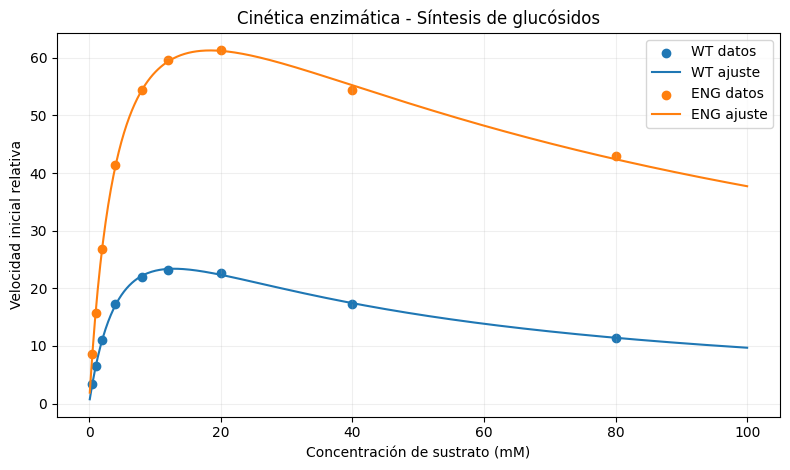
\includegraphics[width=0.43\textwidth]{8.png}}
\\ \hline
\end{tabular}
\caption{Cinética Frente a Concentración de Sustrato}
\caption*{\small\textit{Fuente:} Elaboración propia.}
\end{figure}


\subsection{Respuesta Térmica}
\label{anx:temperatura}

\begin{figure}[H]
\centering
\begin{tabular}{|c|c|}
\hline
\parbox{0.46\textwidth}{\centering\small Procesamiento de Alimentos\\[0.12cm]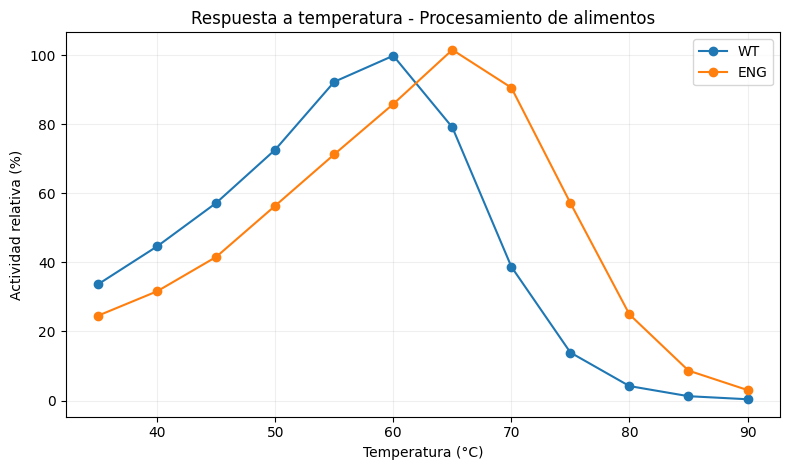
\includegraphics[width=0.43\textwidth]{9.png}}
&
\parbox{0.46\textwidth}{\centering\small Bagazo de Caña\\[0.12cm]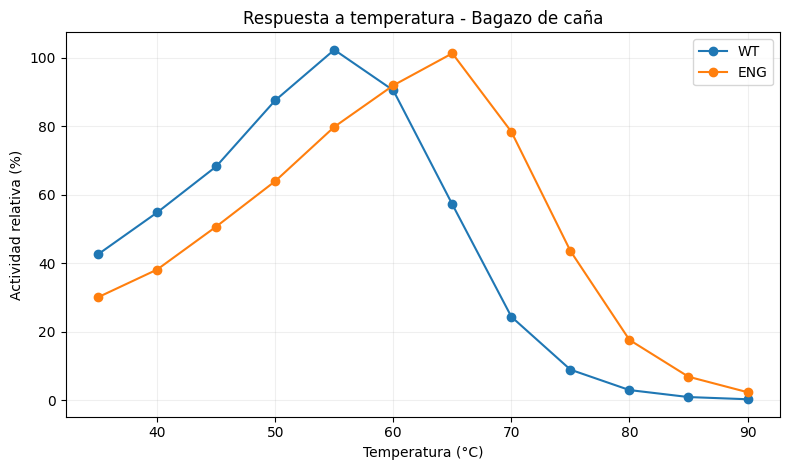
\includegraphics[width=0.43\textwidth]{10.png}}
\\ \hline
\parbox{0.46\textwidth}{\centering\small Procesamiento de Biomasa\\[0.12cm]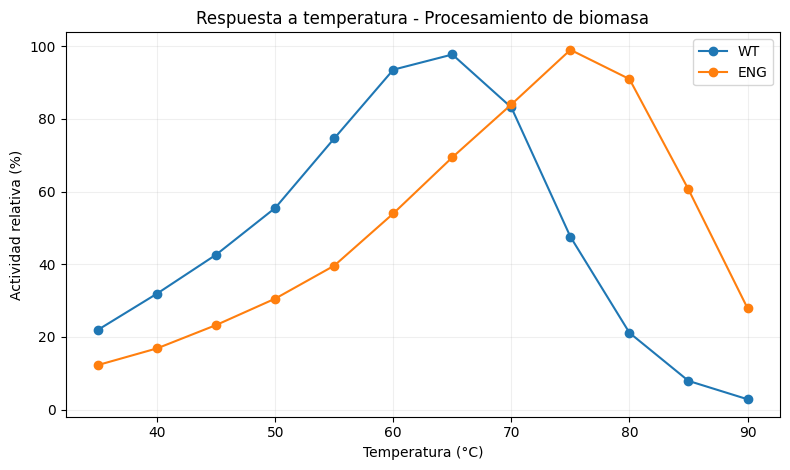
\includegraphics[width=0.43\textwidth]{11.png}}
&
\parbox{0.46\textwidth}{\centering\small Síntesis de Glucósidos\\[0.12cm]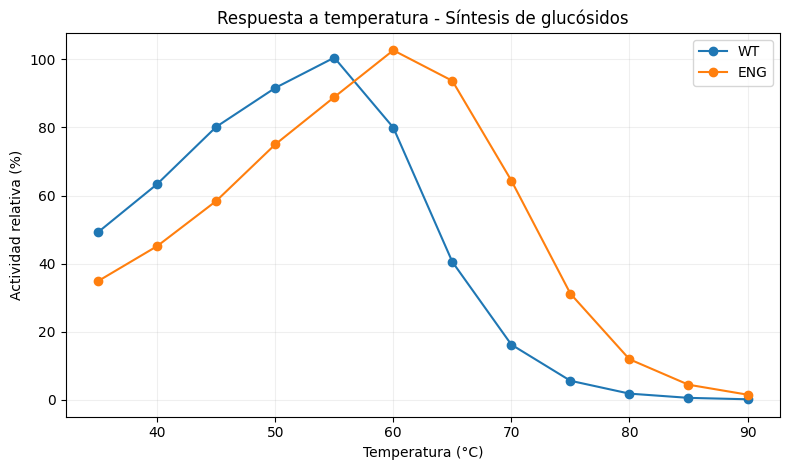
\includegraphics[width=0.43\textwidth]{12.png}}
\\ \hline
\end{tabular}
\caption{Respuesta Térmica}
\caption*{\small\textit{Fuente:} Elaboración propia.}
\end{figure}


\subsection{Selectividad en Síntesis de Glucósidos}
\label{anx:selectividad}

\begin{figure}[H]
\centering
\fbox{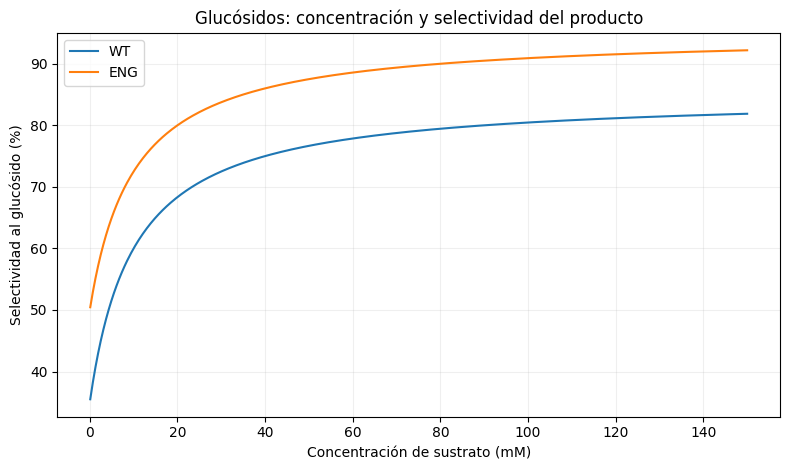
\includegraphics[width=0.65\textwidth]{26.png}}
\caption{Selectividad en Síntesis de Glucósidos}
\caption*{\small\textit{Fuente:} Elaboración propia.}
\end{figure}

\section{Reproducibilidad y Trazabilidad}
\label{sec:reproducibilidad}

\subsection{Condiciones Comunes}
\label{anx:condiciones_repro}
\label{subsec:condiciones_repro}

\begin{table}[H]
\centering
\caption{Condiciones Generales del Análisis}
\caption*{\small\textit{Fuente:} Elaboración propia.}
\label{tab:reproducibilidad}
\renewcommand{\arraystretch}{1.25}
\begin{tabular}{|p{6.0cm}|p{6.2cm}|}
\hline
Condición & Valor \\ \hline
Réplicas & 4 por condición \\ \hline
Evaluación de Estabilidad & \(60\,^{\circ}\mathrm{C}\) \\ \hline
Sustrato en Estabilidad & \(10\,\mathrm{mM}\) \\ \hline
Condición Base de Producción & \(60\,^{\circ}\mathrm{C}\), 40 mM, 8 horas \\ \hline
Rango de Sustrato & \(0.5--80\,\mathrm{mM}\) \\ \hline
Rango de Temperatura & \(35--90\,^{\circ}\mathrm{C}\), pasos de \(5\,^{\circ}\mathrm{C}\) \\ \hline
\end{tabular}
\end{table}

\subsection{Variables Registradas}
\label{anx:variables_repro}
\label{subsec:variables_repro}

\begin{enumerate}
    \item actividad residual durante exposición térmica;
    \item velocidad inicial frente a concentración de sustrato;
    \item actividad relativa frente a temperatura;
    \item producto acumulado durante ocho horas.
\end{enumerate}


\subsection{Indicadores de Comparación}
\label{anx:indicadores_repro}

\begin{equation}
I_S=
\frac{\text{Estabilidad ENG}}
{\text{Estabilidad WT}},
\qquad
I_C=
\frac{\text{Eficiencia ENG}}
{\text{Eficiencia WT}}
\end{equation}

\begin{equation}
I_P=
\frac{\text{Producto ENG}}
{\text{Producto WT}},
\qquad
F_P=
\frac{I_P}{I_S I_C}.
\end{equation}

\(I_S\), \(I_C\) e \(I_P\) mayores que 1 indican mejora frente a WT.
\(F_P<1\) indica que otras restricciones absorben parte de la mejora molecular;
\(F_P>1\) indica que otros factores amplifican el resultado.


\subsection{Funciones Utilizadas}
\label{anx:funciones}
\label{subsec:funciones_repro}

\begin{equation}
A(t)=
A_0
\exp\left[
-\left(
\frac{t}{\tau}
\right)^{\beta}
\right].
\end{equation}

\begin{equation}
v=
\frac{V_{\max}[S]}
{K_m+[S]+\dfrac{[S]^2}{K_i}}.
\end{equation}

\subsection{Trazabilidad del Análisis}
\label{anx:trazabilidad}
\label{subsec:trazabilidad}

\begin{equation}
\text{Medición}
\longrightarrow
\text{Comparación WT--ENG}
\longrightarrow
\text{Resultado Productivo}
\longrightarrow
\text{Punto de Operación}
\longrightarrow
\text{Decisión}.
\end{equation}


\end{document}